\documentclass[../Main.tex]{subfiles}
\begin{document}

This chapter presents the detailed implementation processes of the key components in our integrated AI-powered e-learning system. Building upon the system analysis and design outlined in Chapter \ref{chapter:system_ananlysis_and_design}, we focus on the practical aspects of implementing each system component, highlighting the critical implementation decisions, technical configurations, and integration challenges encountered during development.

The chapter is structured into four main sections, each corresponding to a core system component. In Section \ref{section:5.1_ai_system_implementation}, we detail the implementation of the AI system, with particular emphasis on the customization of the RAGFlow framework for our RAG service. This includes the integration of specialized components for deep document parsing and Vietnamese language processing. Section \ref{section:5.2_e_learning_backend_system_implementation} covers the implementation of the e-learning backend system, focusing on the deployment of OpenEdX in development mode and the implementation of CORS bypassing mechanisms for seamless frontend-backend communication.

Section \ref{section:5.3_e_learning_frontend_system_implementation} presents the implementation of the e-learning frontend system, with special attention to the knowledge citation feature, including PDF rendering and reference visualization capabilities. Finally, Section \ref{section:5.4_developer_tool_implementation} describes the development of essential developer tools, including the OpenAPI2MCP converter and the tool execution history interface.

For each system component, we provide comprehensive details about the project settings, including environment configurations, dependencies, and key hyperparameters. This chapter serves as a practical guide for understanding the technical implementation details of our integrated system.

\section{AI System Implementation}
\label{section:5.1_ai_system_implementation}

As outlined in Section \ref{section:4.1_ai_system_architecture}, our AI system architecture comprises three fundamental components: the Retrieval Service, Tool Ecosystem, and Agentic Workflow. The Inference Provider, while being a crucial component, remains unmodified in our implementation as we leverage existing services. This section focuses on the implementation details of the Retrieval Service and a sample supernet implementation based on the theoretical framework presented in Chapter \ref{chapter:Theoretical_foundation_of_agentic_workflow_framework}.

For the Retrieval Service, we have customized the open-source RAGFlow framework to enhance its capabilities in handling complex document processing and Vietnamese language support. The implementation includes specialized modules for deep document parsing and language tokenization, which are essential for effective information retrieval in our educational context. The Tool Ecosystem implementation, which emphasizes the MCP integration standardized workflow, is detailed separately in Section \ref{section:5.4.2_programming_openapi2mcp_auto_converter}.

The implementation of the Agentic Workflow component demonstrates the practical application of our theoretical framework, featuring a sample supernet design that operationalizes the concepts discussed in Chapter \ref{chapter:Theoretical_foundation_of_agentic_workflow_framework}. This implementation serves as a proof of concept for our proposed theoretical approach to agentic workflow design.

\subsection{Project Settings}
\label{section:5.1.1_project_settings}

\subsection{RAGFlow Customization for RAG Service}
\label{section:5.1.2_ragflow_customization}

RAGFlow is an open-source framework designed for building Retrieval-Augmented Generation (RAG) services, offering a comprehensive solution for document processing, embedding generation, and vector storage. While the framework provides robust capabilities for handling English and Chinese documents, its implementation presents significant limitations when dealing with Vietnamese content. Two critical issues necessitated substantial modifications to the framework:

First, the framework's Optical Character Recognition (OCR) capabilities are specifically optimized for English and Chinese documents, lacking support for Vietnamese character recognition. This limitation significantly impacts the system's ability to process Vietnamese educational materials and documents.

Second, the language tokenization system in RAGFlow employs a dual-approach architecture: NLTK for English text processing and a trie tree-based system for Chinese. For all other languages, including Vietnamese, the framework defaults to using NLTK tokenization, which is not suitable for Vietnamese language characteristics and linguistic rules. This limitation affects the quality of text processing and, consequently, the effectiveness of the retrieval system for Vietnamese content.

To address these limitations, I have implemented custom solutions by integrating specialized Vietnamese language processing tools and document parsing capabilities. The following subsections detail these implementations and their integration with the RAGFlow framework.

\subsubsection{Conda Library Mounting}
\label{section:5.1.2.1_conda_library_mounting}

The implementation of specialized libraries for Vietnamese language processing and document understanding required careful consideration of the containerized environment. The system needs to utilize several key libraries:
\begin{itemize}
    \item \texttt{surya} for advanced document understanding
    \item \texttt{torch} for running Surya's deep learning models
    \item \texttt{underthesea} for Vietnamese language processing
\end{itemize}

To manage these dependencies effectively, a custom Conda environment was created and mounted into the container. This approach offers several advantages:
\begin{itemize}
    \item Persistent storage of installed packages outside the container
    \item Easy package management and version control
    \item Simplified environment replication across different deployments
    \item Reduced container build time by separating package installation from container creation
\end{itemize}

The Docker Compose configuration implements this mounting strategy:

\lstinputlisting[style=htmlcssjs, caption={Docker Compose Configuration for Library Mounting}]{Code/docker-compose.yaml}

This configuration:
\begin{itemize}
    \item Creates a named volume for the Conda environment
    \item Mounts the volume to the container's Python environment path
    \item Ensures persistence of installed packages across container restarts
    \item Maintains isolation between the container and host system
\end{itemize}

The mounted Conda environment allows for easy installation and management of the required libraries while maintaining the container's lightweight nature and ensuring consistent behavior across different deployment environments.

\subsubsection{Surya Integration for Deep Document Parsing}
\label{section:5.1.2.2_surya_integration_for_deep_document_parsing}

Surya is a state-of-the-art document understanding model developed by Microsoft Research, designed to handle complex document layouts and multilingual text recognition. Unlike traditional OCR systems that primarily focus on text extraction, Surya provides comprehensive document understanding capabilities, including layout analysis, table structure recognition, and multilingual text processing. The model's architecture is based on a vision-language transformer that can process both visual and textual information simultaneously, making it particularly effective for handling complex document structures.

The selection of Surya for Vietnamese OCR processing was driven by several key advantages:

\begin{minipage}[t]{0.3\textwidth}
    \begin{figure}[H]
        \includegraphics[width=\textwidth]{Figure/Surya Benchmark.png}
        \caption{Surya OCR Model Benchmarking Results}
        \label{fig:Surya_Benchmarking_Results}
    \end{figure}
\end{minipage}
\hfill
\begin{minipage}[t]{0.7\textwidth}
    \begin{itemize}
        \item \textbf{Multilingual Support}: Surya's training data includes Vietnamese text, making it inherently capable of recognizing Vietnamese characters and diacritical marks, which are crucial for accurate Vietnamese text processing.
        
        \item \textbf{Layout Understanding}: The model's ability to understand document layouts is particularly valuable for educational materials, which often contain complex structures like tables, equations, and multi-column layouts.
        
        \item \textbf{End-to-End Processing}: Surya provides a unified solution for both text recognition and document structure understanding, eliminating the need for multiple specialized tools and reducing processing complexity.
        
        \item \textbf{High Accuracy}: The model demonstrates superior performance in handling various document formats and quality levels, which is essential for processing diverse educational materials.
    \end{itemize}
\end{minipage}

To integrate Surya with RAGFlow, I modified the framework's OCR implementation. The original implementation used a two-stage process with separate text detection and recognition models, as shown in the following code:

\lstinputlisting[style=py, caption=Original OCR Implementation]{Code/ocr_ragflow_old.py}

This implementation downloaded and used the "deepdoc" model from Hugging Face, which was primarily optimized for English and Chinese documents. To replace this with Surya's more capable document understanding system, I modified the code to use Surya's unified detection and recognition pipeline:

\lstinputlisting[style=py, caption=Modified OCR Implementation]{Code/ocr_ragflow_new.py}

This modification significantly improves the system's ability to process Vietnamese documents while maintaining compatibility with RAGFlow's existing document processing workflow.

\subsubsection{Ubderthesea Integration for Vietnamese NLP}
\label{section:5.1.2.3_ubderthesea_integration_for_vietnamese_nlp}

Underthesea is a comprehensive Vietnamese Natural Language Processing (NLP) toolkit that provides various linguistic analysis capabilities specifically designed for Vietnamese text. The toolkit offers a range of features including word tokenization, part-of-speech tagging, named entity recognition, and sentiment analysis, all optimized for the Vietnamese language's unique characteristics such as its complex diacritical marks and compound words.

The selection of Underthesea for Vietnamese text processing was driven by several key advantages:

\begin{itemize}
    \item \textbf{Vietnamese-Specific Design}: Unlike general-purpose NLP tools, Underthesea is specifically designed to handle Vietnamese language characteristics, including proper handling of diacritical marks and compound words.
    
    \item \textbf{Comprehensive Features}: The toolkit provides a complete suite of NLP tools necessary for text processing, from basic tokenization to advanced linguistic analysis.
    
    \item \textbf{Active Development}: Being an open-source project with active maintenance, Underthesea regularly incorporates improvements and updates for Vietnamese language processing.
    
    \item \textbf{High Accuracy}: The toolkit demonstrates superior performance in handling Vietnamese text compared to general-purpose NLP tools.
\end{itemize}

The original RAGFlow implementation presented significant limitations for Vietnamese text processing. The framework's tokenization system employs a dual-approach architecture:

\begin{itemize}
    \item For English text: Uses NLTK (Natural Language Toolkit) tokenization
    \item For Chinese text: Uses a specialized trie tree-based tokenizer
    \item For all other languages: Defaults to NLTK tokenization
\end{itemize}

To understand how to properly integrate Vietnamese language processing, I first analyzed RAGFlow's English text processing pipeline. The English implementation uses a combination of stemming and lemmatization for text normalization:

\lstinputlisting[style=py, caption=English Text Processing in RAGFlow]{Code/ragflow_eng_tokenizer.py}

This implementation demonstrates that RAGFlow employs a sophisticated approach to English text processing, combining both stemming and lemmatization to reduce words to their base forms. However, this approach is not suitable for Vietnamese due to the language's different morphological characteristics.

For Vietnamese text processing, the primary concern is word segmentation rather than stemming or lemmatization. Vietnamese is an isolating language where words are not inflected, and the main challenge is determining word boundaries in the continuous text. Therefore, I implemented a Vietnamese-specific processing pipeline using Underthesea's word segmentation capabilities, which is more appropriate for the language's characteristics.

\subsection{Simple Supernet for Agentic Workflow}
\label{section:5.1.3_simple_supernet_for_agentic_workflow}

Building upon the theoretical framework presented in Chapter \ref{chapter:Theoretical_foundation_of_agentic_workflow_framework}, this section details the implementation of a practical supernet architecture for agentic workflows. The implementation focuses on creating a 5x5 supernet that incorporates five distinct reasoning operators: Chain-of-Thought (CoT), Debate, ReAct, Self-Consistency, and Early Exit. This design choice was made to demonstrate the practical application of the theoretical concepts while maintaining a manageable scope for implementation.

\subsubsection{Operator Definitions}
\label{section:5.1.3.1_operator_definitions}

The implementation of each reasoning operator follows established research methodologies while being adapted to our specific use case. Below is a detailed description of each operator's implementation:

\paragraph{Chain-of-Thought (CoT)} This operator implements the methodology proposed in "Automatic Chain of Thought Prompting in Large Language Models". The operator functions as a planner, utilizing a few-shot learning approach where relevant examples are retrieved from the knowledge library and incorporated into the prompt. The implementation uses GPT-4 as the primary language model, which is prompted to engage in step-by-step reasoning. The operator's architecture consists of:

\begin{itemize}
    \item \textbf{LLM Component}: GPT-4o serves as the main reasoning engine
    \item \textbf{Tool Component}: A demonstration sampling system that retrieves relevant examples from the knowledge library using RAG technology
\end{itemize}

\paragraph{Debate} Following the framework outlined in "Improving Factuality and Reasoning in Language Models through Multiagent Debate", this operator enables collaborative problem-solving through structured debate among multiple language models. The implementation initializes three debater agents and allows for up to two rounds of debate, leveraging diverse perspectives to arrive at optimal solutions. The operator's architecture consists of:

\begin{itemize}
    \item \textbf{LLM Component}: GPT-4o serves as the main reasoning engine for all debaters
    \item \textbf{Tool Component}: No tool component is required for this operator
\end{itemize}

\paragraph{Self-Consistency} This operator implements the methodology from "Self-Consistency Improves Chain of Thought Reasoning in Language Models". The implementation generates five distinct Chain-of-Thought reasoning paths and employs majority voting to determine the final answer. The operator's architecture consists of:

\begin{itemize}
    \item \textbf{LLM Component}: GPT-4o serves as the main reasoning engine
    \item \textbf{Tool Component}: No tool component is required for this operator
\end{itemize}

\paragraph{ReAct} Following the framework proposed in "ReAct: Synergizing Reasoning and Acting in Language Models", this operator enables the agent to interact with external tools while maintaining reasoning capabilities. The implementation allows the agent to leverage the integrated MCP tools to handle diverse user requirements. The operator's architecture consists of:

\begin{itemize}
    \item \textbf{LLM Component}: GPT-4o serves as the main reasoning engine
    \item \textbf{Tool Component}: All integrated MCP tools are available for the agent to utilize
\end{itemize}

\paragraph{Early Exit} This operator implements a dynamic depth control mechanism for the multi-agent architecture. It interrupts the sampling process when certain conditions are met, enabling the depth of the agentic supernet to be query-dependent. This approach optimizes computational resources by preventing unnecessary processing when a satisfactory solution has been reached. The operator's architecture consists of:

\begin{itemize}
    \item \textbf{LLM Component}: No LLM component is required for this operator
    \item \textbf{Tool Component}: No tool component is required for this operator
\end{itemize}

Each operator is designed to be modular and can be combined with others in the supernet architecture to create complex reasoning workflows. The implementation ensures that each operator maintains its core functionality while being adaptable to different use cases and requirements.

\subsubsection{Supernet Design}
\label{section:5.1.3.2_supernet_design}
The supernet architecture is designed as a 5x5 network, comprising five layers with five operators in each layer. This design choice was made based on two key considerations:


\begin{itemize}
    \item \textbf{Operator Selection}: The five operators (CoT, Debate, ReAct, Self-Consistency, and Early Exit) were chosen to provide a comprehensive set of reasoning capabilities while maintaining a manageable implementation scope.
    
    \item \textbf{Layer Depth}: The five-layer architecture was designed to accommodate the longest possible reasoning path that could traverse all operators, ensuring the system can handle complex queries requiring multiple reasoning steps.
\end{itemize}

The supernet implements a query-dependent path selection mechanism, where the complexity of the query is determined by its length. This approach ensures that the system allocates appropriate computational resources based on the query's complexity. The path selection follows these rules:

\begin{minipage}[t]{0.6\textwidth}
\begin{itemize}
    \item \textbf{Easy Queries} (less than 7 words): Utilizes a minimal path of ReAct > Early Exit, providing quick responses for straightforward queries.
    
    \item \textbf{Moderate Queries} (7-21 words): Follows the path CoT > ReAct > Early Exit, adding step-by-step reasoning for more complex queries.
    
    \item \textbf{Complex Queries} (22-35 words): Implements the path Debate > CoT > ReAct > Early Exit, incorporating multiple perspectives through debate for intricate queries.
    
    \item \textbf{Highly Complex Queries} (more than 35 words): Employs the full path Debate > CoT > ReAct > Self-Consistency > Early Exit, utilizing all reasoning capabilities for the most demanding queries.
\end{itemize}

\end{minipage}
\hfill
\begin{minipage}[t]{0.35\textwidth}
\begin{figure}[H]
    \centering
    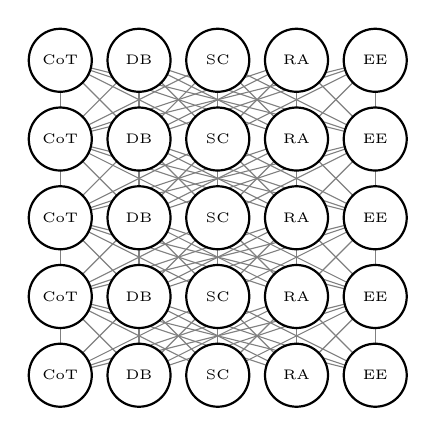
\begin{tikzpicture}[
        node distance=1cm,
        operator/.style={circle, draw=black, minimum size=0.8cm, thick, inner sep=0pt, fill=white},
        connection/.style={-, gray, thin}
    ]
        % Connections between layers (drawn first)
        \foreach \i in {0,...,4} {
            \foreach \j in {0,...,4} {
                \draw[connection] (\i*1cm, 0) -- (\j*1cm, -1cm);
                \draw[connection] (\i*1cm, -1cm) -- (\j*1cm, -2cm);
                \draw[connection] (\i*1cm, -2cm) -- (\j*1cm, -3cm);
                \draw[connection] (\i*1cm, -3cm) -- (\j*1cm, -4cm);
            }
        }
        
        % Nodes (drawn last, with labels inside)
        \foreach \x in {0,...,4} {
            \node[operator] at (\x*1cm, 0) {\tiny \ifcase\x CoT\or DB\or SC\or RA\or EE\fi};
            \node[operator] at (\x*1cm, -1cm) {\tiny \ifcase\x CoT\or DB\or SC\or RA\or EE\fi};
            \node[operator] at (\x*1cm, -2cm) {\tiny \ifcase\x CoT\or DB\or SC\or RA\or EE\fi};
            \node[operator] at (\x*1cm, -3cm) {\tiny \ifcase\x CoT\or DB\or SC\or RA\or EE\fi};
            \node[operator] at (\x*1cm, -4cm) {\tiny \ifcase\x CoT\or DB\or SC\or RA\or EE\fi};
        }
    \end{tikzpicture}
    \caption{Supernet Architecture with Five Operators}
    \label{fig:supernet_architecture}
\end{figure}
\end{minipage}

This design ensures that:
\begin{itemize}
    \item The system can handle queries of varying complexity efficiently
    \item Computational resources are allocated proportionally to query complexity
    \item The reasoning process is appropriately structured for each query type
    \item The system maintains flexibility while providing consistent performance
\end{itemize}

The supernet's architecture allows for dynamic path selection based on query characteristics, ensuring optimal performance while maintaining the system's ability to handle complex reasoning tasks.


\section{E-learning Backend System Implementation}
\label{section:5.2_e_learning_backend}

The implementation of the e-learning backend system is centered around OpenEdX, a robust and scalable learning management platform. This section details the deployment and configuration of the OpenEdX backend using Tutor, an open-source platform management tool developed by edly.io. The implementation process encompasses several critical aspects, including the initial setup of the OpenEdX environment, configuration of the learning management system, and the resolution of cross-origin resource sharing (CORS) restrictions. Given the distributed nature of the system, where the frontend and backend components operate on different ports, particular attention was paid to ensuring secure and efficient communication between these components. The implementation strategy focuses on maintaining system integrity while enabling seamless interaction between the frontend interface and the backend services.

\subsection{Project Settings}
\label{section:5.2.1_project_settings}

\subsection{Running OpenEdX Backend in Development Mode}
\label{section:5.2.2_running_openedx_backend_in_development_mode}
The development environment for OpenEdX was established using Tutor, which provides a streamlined approach to deploying and managing OpenEdX instances. The standard development setup process involves three primary steps:

\begin{enumerate}
    \item Mounting the local edx-platform directory: \texttt{tutor mounts add ./edx-platform}
    \item Building the development Docker image: \texttt{tutor images build openedx-dev}
    \item Launching the development environment: \texttt{tutor dev launch}
\end{enumerate}

However, the initial implementation attempt encountered a version compatibility issue. This occurred because the edx-platform repository was cloned from the master branch, while the installed Tutor version was specifically designed to work with the Sumac branch of OpenEdX. This incompatibility arose from the fact that Tutor maintains specific version alignments between its deployment tools and the OpenEdX platform code to ensure stability and compatibility of all components.

The version mismatch manifested as build errors during the image construction phase, as the master branch contained code structures and dependencies that were not compatible with the Tutor configuration. This is a common challenge in OpenEdX development, as the platform's architecture requires precise version alignment between its various components.

The issue was resolved by switching the edx-platform repository to the Sumac branch, which is the version that Tutor was configured to support. This alignment ensured that all components, including the platform code, Docker configurations, and deployment scripts, were compatible with each other. The successful implementation following this version adjustment demonstrates the importance of maintaining version consistency in the OpenEdX ecosystem.

\subsection{CORS Bypassing With Plugin}
\label{section:5.2.3_cors_bypassing_with_plugin}

The implementation of the e-learning system required the frontend and backend components to operate on different ports, with the NextJS frontend running on port 3000 and the OpenEdX backend on port 8000. This separation led to cross-origin resource sharing (CORS) restrictions, which prevented the frontend from making API calls to the backend. The browser's security policy blocked these cross-origin requests, resulting in "Cross-Origin Request Blocked" errors.

To resolve this issue, a custom plugin was developed to modify OpenEdX's CORS configuration. The plugin adds the frontend's origin (http://localhost:3000) to both the CORS\_ORIGIN\_WHITELIST and CSRF\_TRUSTED\_ORIGINS environment variables. This configuration allows the frontend to make authenticated requests to the backend while maintaining security standards.

The plugin implementation is shown below:

\lstinputlisting[style=py, caption={CORS Configuration Plugin for OpenEdX}]{Code/cors_plugin.py}

This solution ensures that:
\begin{itemize}
    \item The frontend can make API calls to the backend without CORS restrictions
    \item CSRF protection remains active for security
    \item The configuration is applied consistently across the OpenEdX platform
    \item The development environment maintains proper security standards while allowing necessary cross-origin communication
\end{itemize}

The plugin approach was chosen over direct configuration file modifications because it provides a more maintainable and portable solution. This implementation allows the CORS settings to persist across platform updates and can be easily deployed to different environments.

\section{E-learning Frontend System Implementation}
\label{section:5.3_e_learning_frontend_system_implementation}

The frontend implementation of the e-learning system focuses on creating an intuitive and interactive user interface that seamlessly integrates with the backend services (including OpenEdX and AI System). This section will focus on the key feature of this implementation, which is the Knowledge Citation system. This functionality enhances the user experience by providing visual context for AI-generated responses. This system automatically identifies and highlights relevant sections within source documents, creating a transparent connection between the AI's responses and the underlying knowledge base.


\subsection{Project Settings}
\label{section:5.3.1_project_settings}
\subsection{Programming Document Preview Interface}
\label{section:5.3.2_programming_document_preview_interface}

The document preview interface was implemented using \texttt{react-pdf}, a React component that provides programmatic control over PDF rendering. This choice was made over traditional iframe-based PDF viewers to enable precise overlay rendering of citation boxes on the document content. The implementation leverages the canvas-based rendering capabilities of react-pdf, allowing for dynamic drawing of visual elements on top of the PDF content.

The citation system consists of two main components: spatial information storage and visual rendering. During the document indexing process, each text chunk's spatial information is captured and stored in a structured format:

\begin{itemize}
    \item The page number where the chunk appears
    \item The bounding box coordinates \texttt{[x1, y1, x2, y2]} defining the chunk's position within the page
\end{itemize}

This spatial metadata is attached to the retrieved chunks during the RAG process, enabling precise citation visualization. The implementation handles the coordinate system transformation between the stored bounding box coordinates and the canvas space, ensuring accurate placement of citation boxes regardless of the PDF's display size or zoom level.

The citation system processes a position array of five integers:
\begin{itemize}
    \item First integer: Page number
    \item Remaining four integers: Bounding box coordinates \texttt{[x1, y1, x2, y2]}
\end{itemize}

These coordinates are used to define the four corners of the citation box on the canvas. The implementation includes two key features:

\begin{enumerate}
    \item \textbf{Citation Box Drawing}: Dynamically renders citation boxes on the PDF canvas using the stored coordinates
    \item \textbf{Auto-scrolling}: Automatically navigates to the relevant page when a citation is referenced
\end{enumerate}

The implementation of these features is shown in the following code snippets:

\lstinputlisting[style=htmlcssjs, caption={Knowledge Citation Box Drawing}]{Code/knowledge_citation.js}

\lstinputlisting[style=htmlcssjs, caption={Auto Scroll}]{Code/auto_scrolling.js}

This implementation ensures that users can easily trace the source of information in the AI-generated responses, enhancing the transparency and reliability of the system.

\section{Developer Tool Implementation}
\label{section:5.4_developer_tool_implementation}

The implementation of developer tools focuses on streamlining the integration of external services into the AI system through the MCP (Machine-Callable Protocol) framework. A key component of this implementation is the OpenAPI2MCP Auto-Converter, which automates the transformation of OpenAPI specifications into MCP-compatible server implementations. This tool employs a template-based approach, where a predefined MCP Server JavaScript project structure serves as the foundation. The converter systematically parses OpenAPI YAML specifications, extracting endpoint definitions, parameters, and response schemas, then generates corresponding MCP server code by injecting the parsed information into the template structure. This automated conversion process significantly reduces the development effort required to integrate new services into the AI system while ensuring consistency in the implementation of MCP servers.

\subsection{Project Settings}
\label{section:5.4.1_project_settings}
\subsection{Programming OpenAPI2MCP Auto-Converter}
\label{section:5.4.2_programming_openapi2mcp_auto_converter}

The OpenAPI2MCP Auto-Converter is implemented as a modular system that transforms OpenAPI specifications into MCP-compatible server code. The conversion process is structured around three main template generators, each responsible for a specific aspect of the MCP server implementation:

\begin{enumerate}
    \item \textbf{Tool Handling Generator}: Creates the core request handling logic for each API endpoint. This generator processes the OpenAPI path definitions and generates corresponding route handlers that implement the MCP protocol's request-response flow.
    
    \item \textbf{Tool Definition Generator}: Generates the MCP tool definitions that describe the available operations, their parameters, and return types. This component ensures that the generated server properly exposes the API functionality in a format that the AI system can understand and utilize.
    
    \item \textbf{Security Code Generator}: Implements the necessary authentication and authorization mechanisms based on the OpenAPI security schemes. This generator ensures that the MCP server properly handles API keys, OAuth tokens, or other security requirements specified in the OpenAPI document.
\end{enumerate}

The template structure for each generator is shown below:

\lstinputlisting[style=htmlcssjs, caption={Tool Handling Template}]{Code/tool_handling_template.js}

\lstinputlisting[style=htmlcssjs, caption={Tool Definition Template}]{Code/tool_definition_template.js}

\lstinputlisting[style=htmlcssjs, caption={Security Code Template}]{Code/security_template.js}

The conversion process follows these steps:
\begin{enumerate}
    \item Parse the OpenAPI YAML specification using a YAML parser
    \item Extract endpoint definitions, parameters, and security requirements
    \item For each endpoint:
    \begin{itemize}
        \item Generate tool handling code using the template
        \item Create corresponding tool definition
        \item Implement required security measures
    \end{itemize}
    \item Combine all generated code into a complete MCP server implementation
    \item Generate necessary configuration files and dependencies
\end{enumerate}

This modular approach allows for:
\begin{itemize}
    \item Consistent implementation of MCP servers across different APIs
    \item Easy maintenance and updates of the conversion process
    \item Flexible handling of different API structures and security requirements
    \item Automated generation of type-safe and well-documented code
\end{itemize}

The generated MCP server can be immediately built and deployed, providing a seamless integration point for the AI system to interact with the original API.
\end{document}